\section{Result}
After three months of development, the APIs and Dashboard for Data Lake has basically been completed, meeting the initial criteria. To be more specific, a website has been designed with the following functions:
\begin{itemize}
    \item \textbf{Register and Login}: Allows users to create an account and log in using the registered account based on username and a real email.
    \item \textbf{Manage Users}: Allow Admin to read, create, edit, and delete information about users.
    \item \textbf{Manage User Groups}: Allow Admin to read, create, edit, and delete information about groups.
    \item \textbf{Manage Folders and Manage Files}: Authorized users are allowed to read, create, edit, and delete information about files and folders. To increase productivity, users can filter them by custom criteria.
    \item \textbf{Manage ACLs}: Authorized users are allowed to grant permission for other users on the files or folders they selected.
\end{itemize}

\subsection{API}
These are all the endpoints for the API we have been building: 
\begin{longtable}{|p{2cm}|p{5cm}|p{5cm}|}
\caption{All API Endpoints}
\label{table:APIendpoints} \\

\hline \multicolumn{1}{|c|}{\textbf{Methods}} & \multicolumn{1}{c|}{\textbf{URLs}} & \multicolumn{1}{c|}{\textbf{Action}} \\ \hline 
\endfirsthead
  \hline 
POST & /api/auth/signup & Signup new account\\ \hline
POST & /api/auth/signin & Login an account\\ \hline
POST & /api/auth/refresh-token & Get access token from refresh token \\ \hline
GET & /api/auth/logout & Logout current user\\ \hline
GET & /api/users/check\_email & Check if Email is available to use \\ \hline
GET &
/api/users/my-profile &
Get the logged in's user profile \\ \hline

GET &
/api/users/\{id\} &
Get user by ID \\ \hline

PUT &
/api/users/\{id\} &
Update user by ID \\ \hline

DELETE &
/api/users/\{id\} &
Delete user by ID \\ \hline

GET &
/api/users/check\_username &
Check if Username is available to use \\ \hline

GET &
/api/users/find/{username} &
Get user by user name \\ \hline

GET &
/api/users &
Get a list of all users in the system \\ \hline

GET &
/api/groups/\{id\} &
Get a group by ID \\ \hline

DELETE &
/api/groups/\{id\} &
Delete a group \\ \hline

PUT &
/api/groups/\{groupId\}/users/ \newline\{username\} &
Add a user to a group \\ \hline

GET &
/api/groups/find/\{name\} &
Get a group by name \\ \hline

GET &
/api/groups &
Get all groups \\ \hline

POST &
/api/groups &
Add an user group \\ \hline

GET &
/api/find/name/\{name\} &
Find all files and folders by name containing \\ \hline

GET &
/api/find/topics &
Get files and folders by topics \\ \hline

GET &
/api/folders/ls/\{folderId\} &
List all files and subfolders inside the folder by ID \\ \hline

GET &
/api/content &
Get all first node files and folders \\ \hline

GET & 
/api/folders &
Get all folders \\ \hline

POST & 
/api/folders &
Add a folder \\ \hline

GET & 
/api/folders/\{id\} &
Get a folder by ID \\ \hline

PUT & 
/api/folders/\{id\} &
Update a folder by ID \\ \hline

DELETE & 
/api/folders/\{id\} &
Delete a folder \\ \hline

GET & 
/api/folders/content/\{id\} &
Get a list of content inside folder by ID \\ \hline

PUT & 
/api/folders/\{folderId\}/\newline subfolders/\{subfolderId\} &
Add a subfolder to folder \\ \hline

PUT & 
/api/folders/\{folderId\}/files/\newline\{fileId\} &
Add a file to a folder \\ \hline

GET &
/api/files/data/\{id\} &
Get File Data \\ \hline

GET &
/api/files/\{id\} &
Get a file by ID \\ \hline

PUT &
/api/files/\{id\} &
Update a file by ID \\ \hline

DELETE &
/api/files/\{id\} &
Delete a file by ID \\ \hline

GET &
/api/folder/\{folderId\}/files &
Get All Files by Folder Id \\ \hline

GET &
/api/files &
Get all files \\ \hline

POST & 
/api/files &
Upload a file \\ \hline

PUT &
/api/acl/file/user &
Grant File Permission For User \\ \hline

DELETE &
/api/acl/file/user &
Remove a File Permission For User \\ \hline

GET &
/api/acl/perm &
Get All Permissions \\ \hline

PUT &
/api/acl/folder/user &
Grant Folder Permission For User \\ \hline

DELETE &
/api/acl/folder/user &
Remove a File Permission For User \\ \hline

PUT &
/api/acl/file/group &
Grant File Permission For Group \\ \hline

DELETE &
/api/acl/file/group &
Remove a File Permission For Group \\ \hline

PUT &
/api/acl/folder/group &
Grant Folder Permission For Group \\ \hline

DELETE &
/api/acl/folder/group &
Remove a Folder Permission For Group \\ \hline
\end{longtable}

\subsection{Web Dashboard}
Following are the screenshots for the Manage Files Use Case, of the Web Dashboard we have been building. The rest is included in the Appendices section. 
\begin{figure}[H]
    \centering
    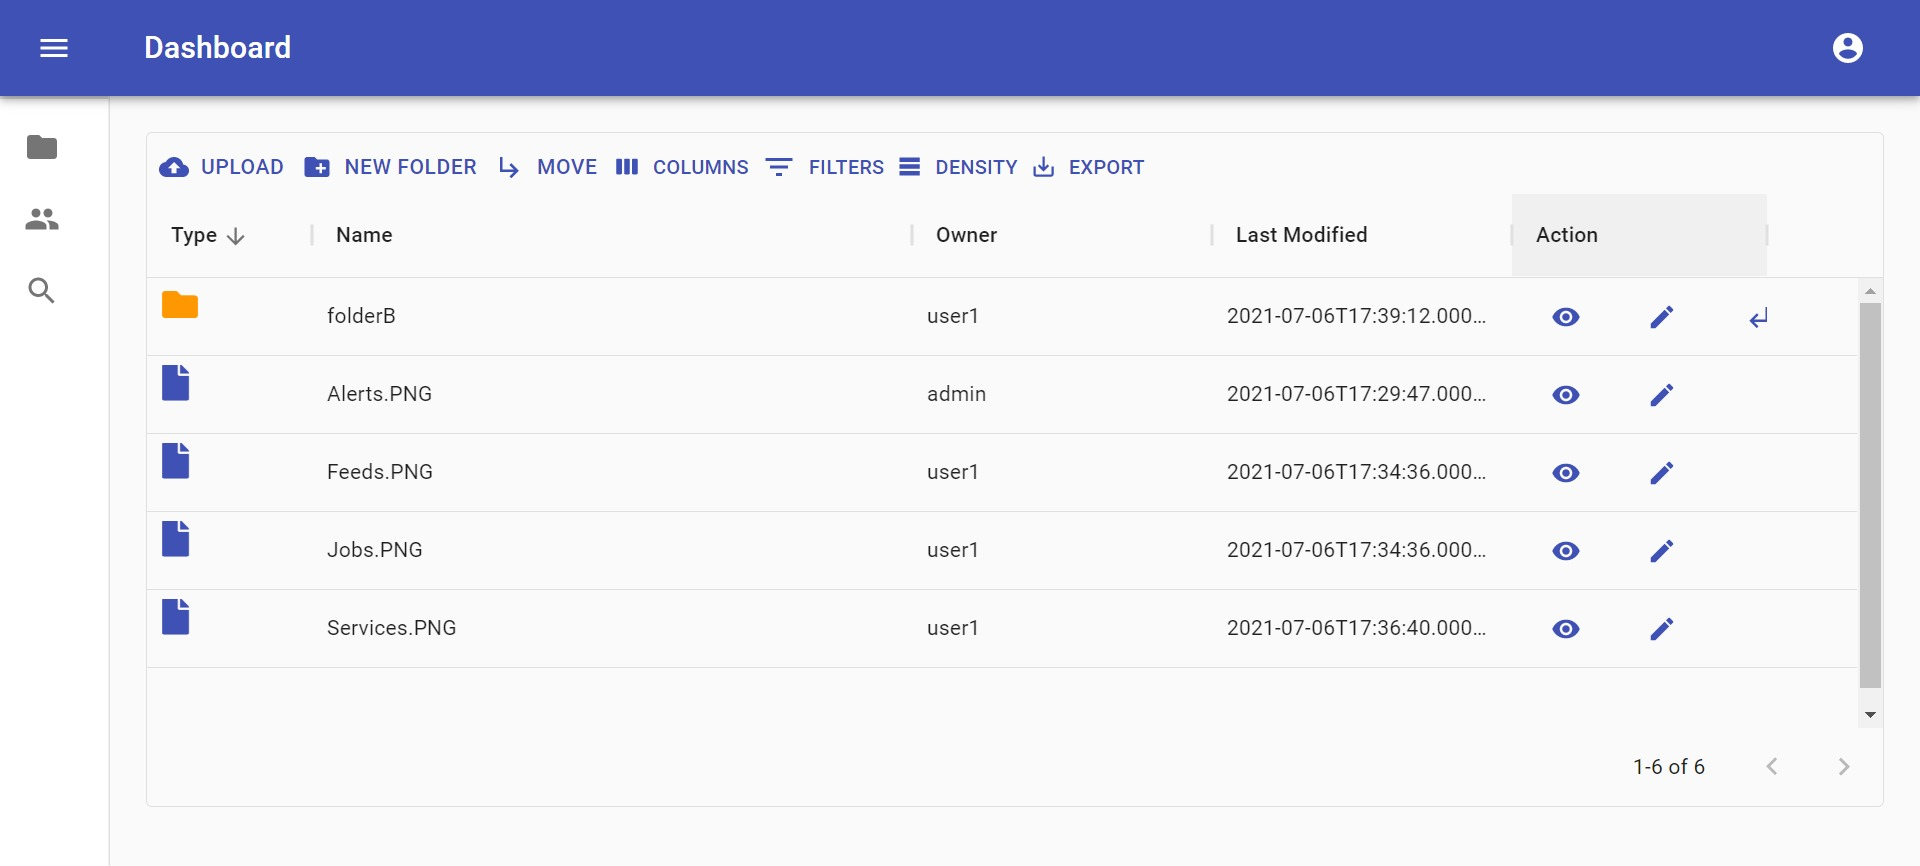
\includegraphics[width=1.0\textwidth]{images/Directory-Listing.jpg}
    \caption{List all files and folders user interface}
    \label{fig:listContent}
\end{figure}
\begin{figure}[H]
    \centering
    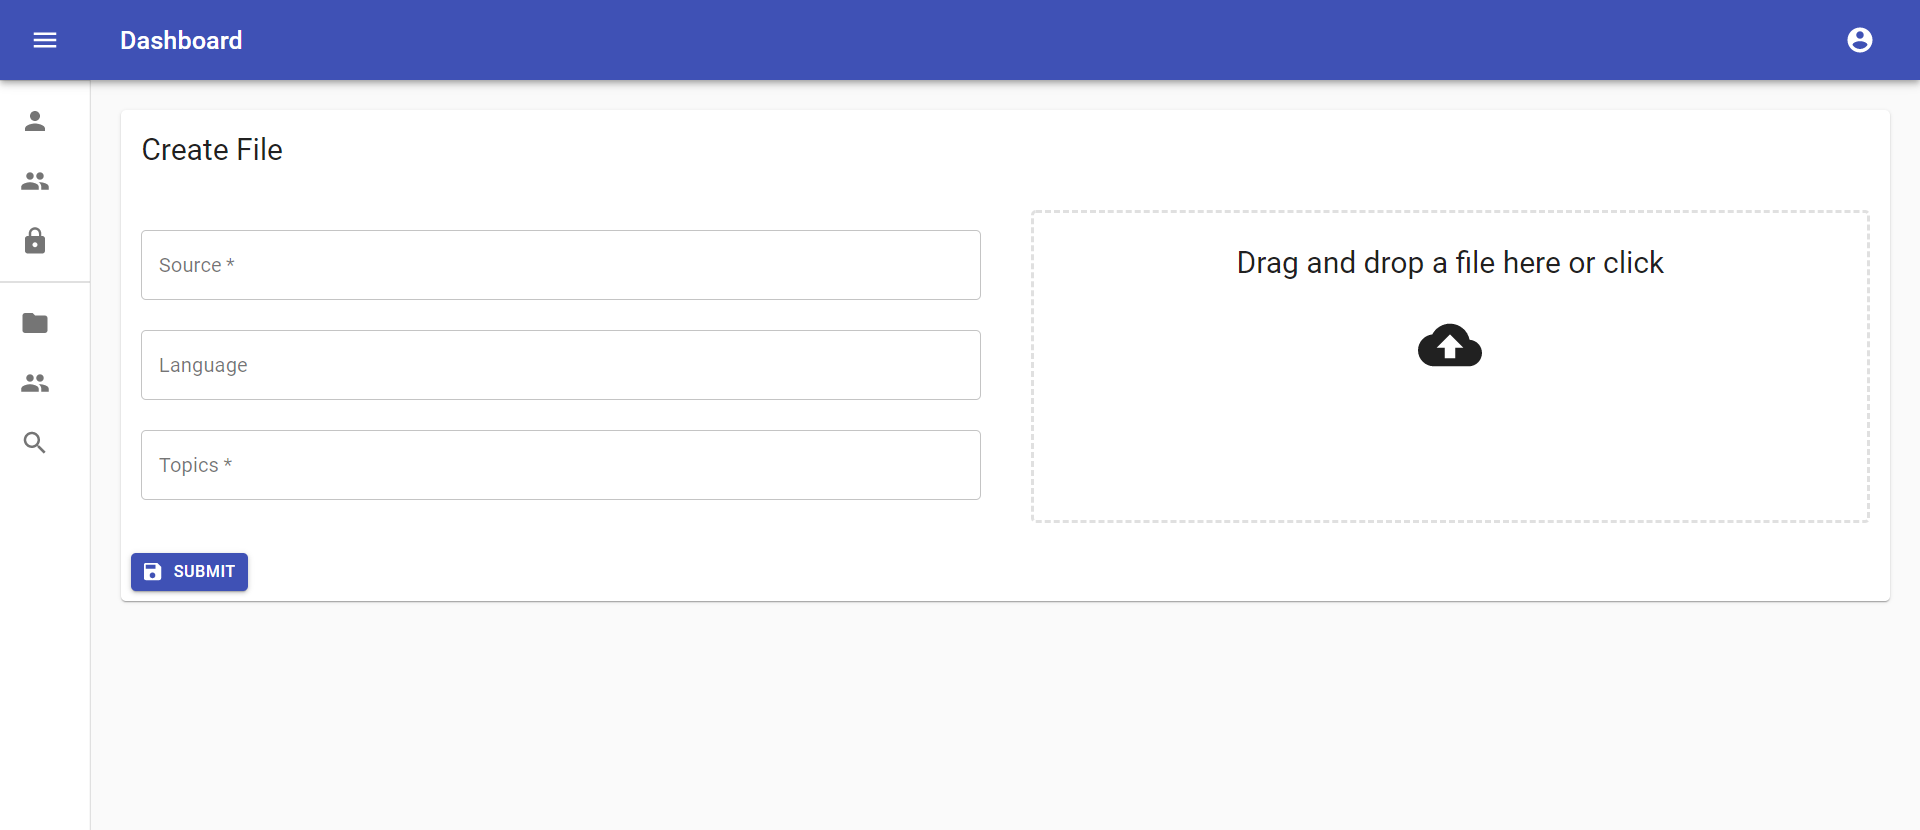
\includegraphics[width=1.0\textwidth]{images/File-Upload.png}
    \caption{Upload File user interface}
    \label{fig:uploadFile}
\end{figure}
\begin{figure}[H]
    \centering
    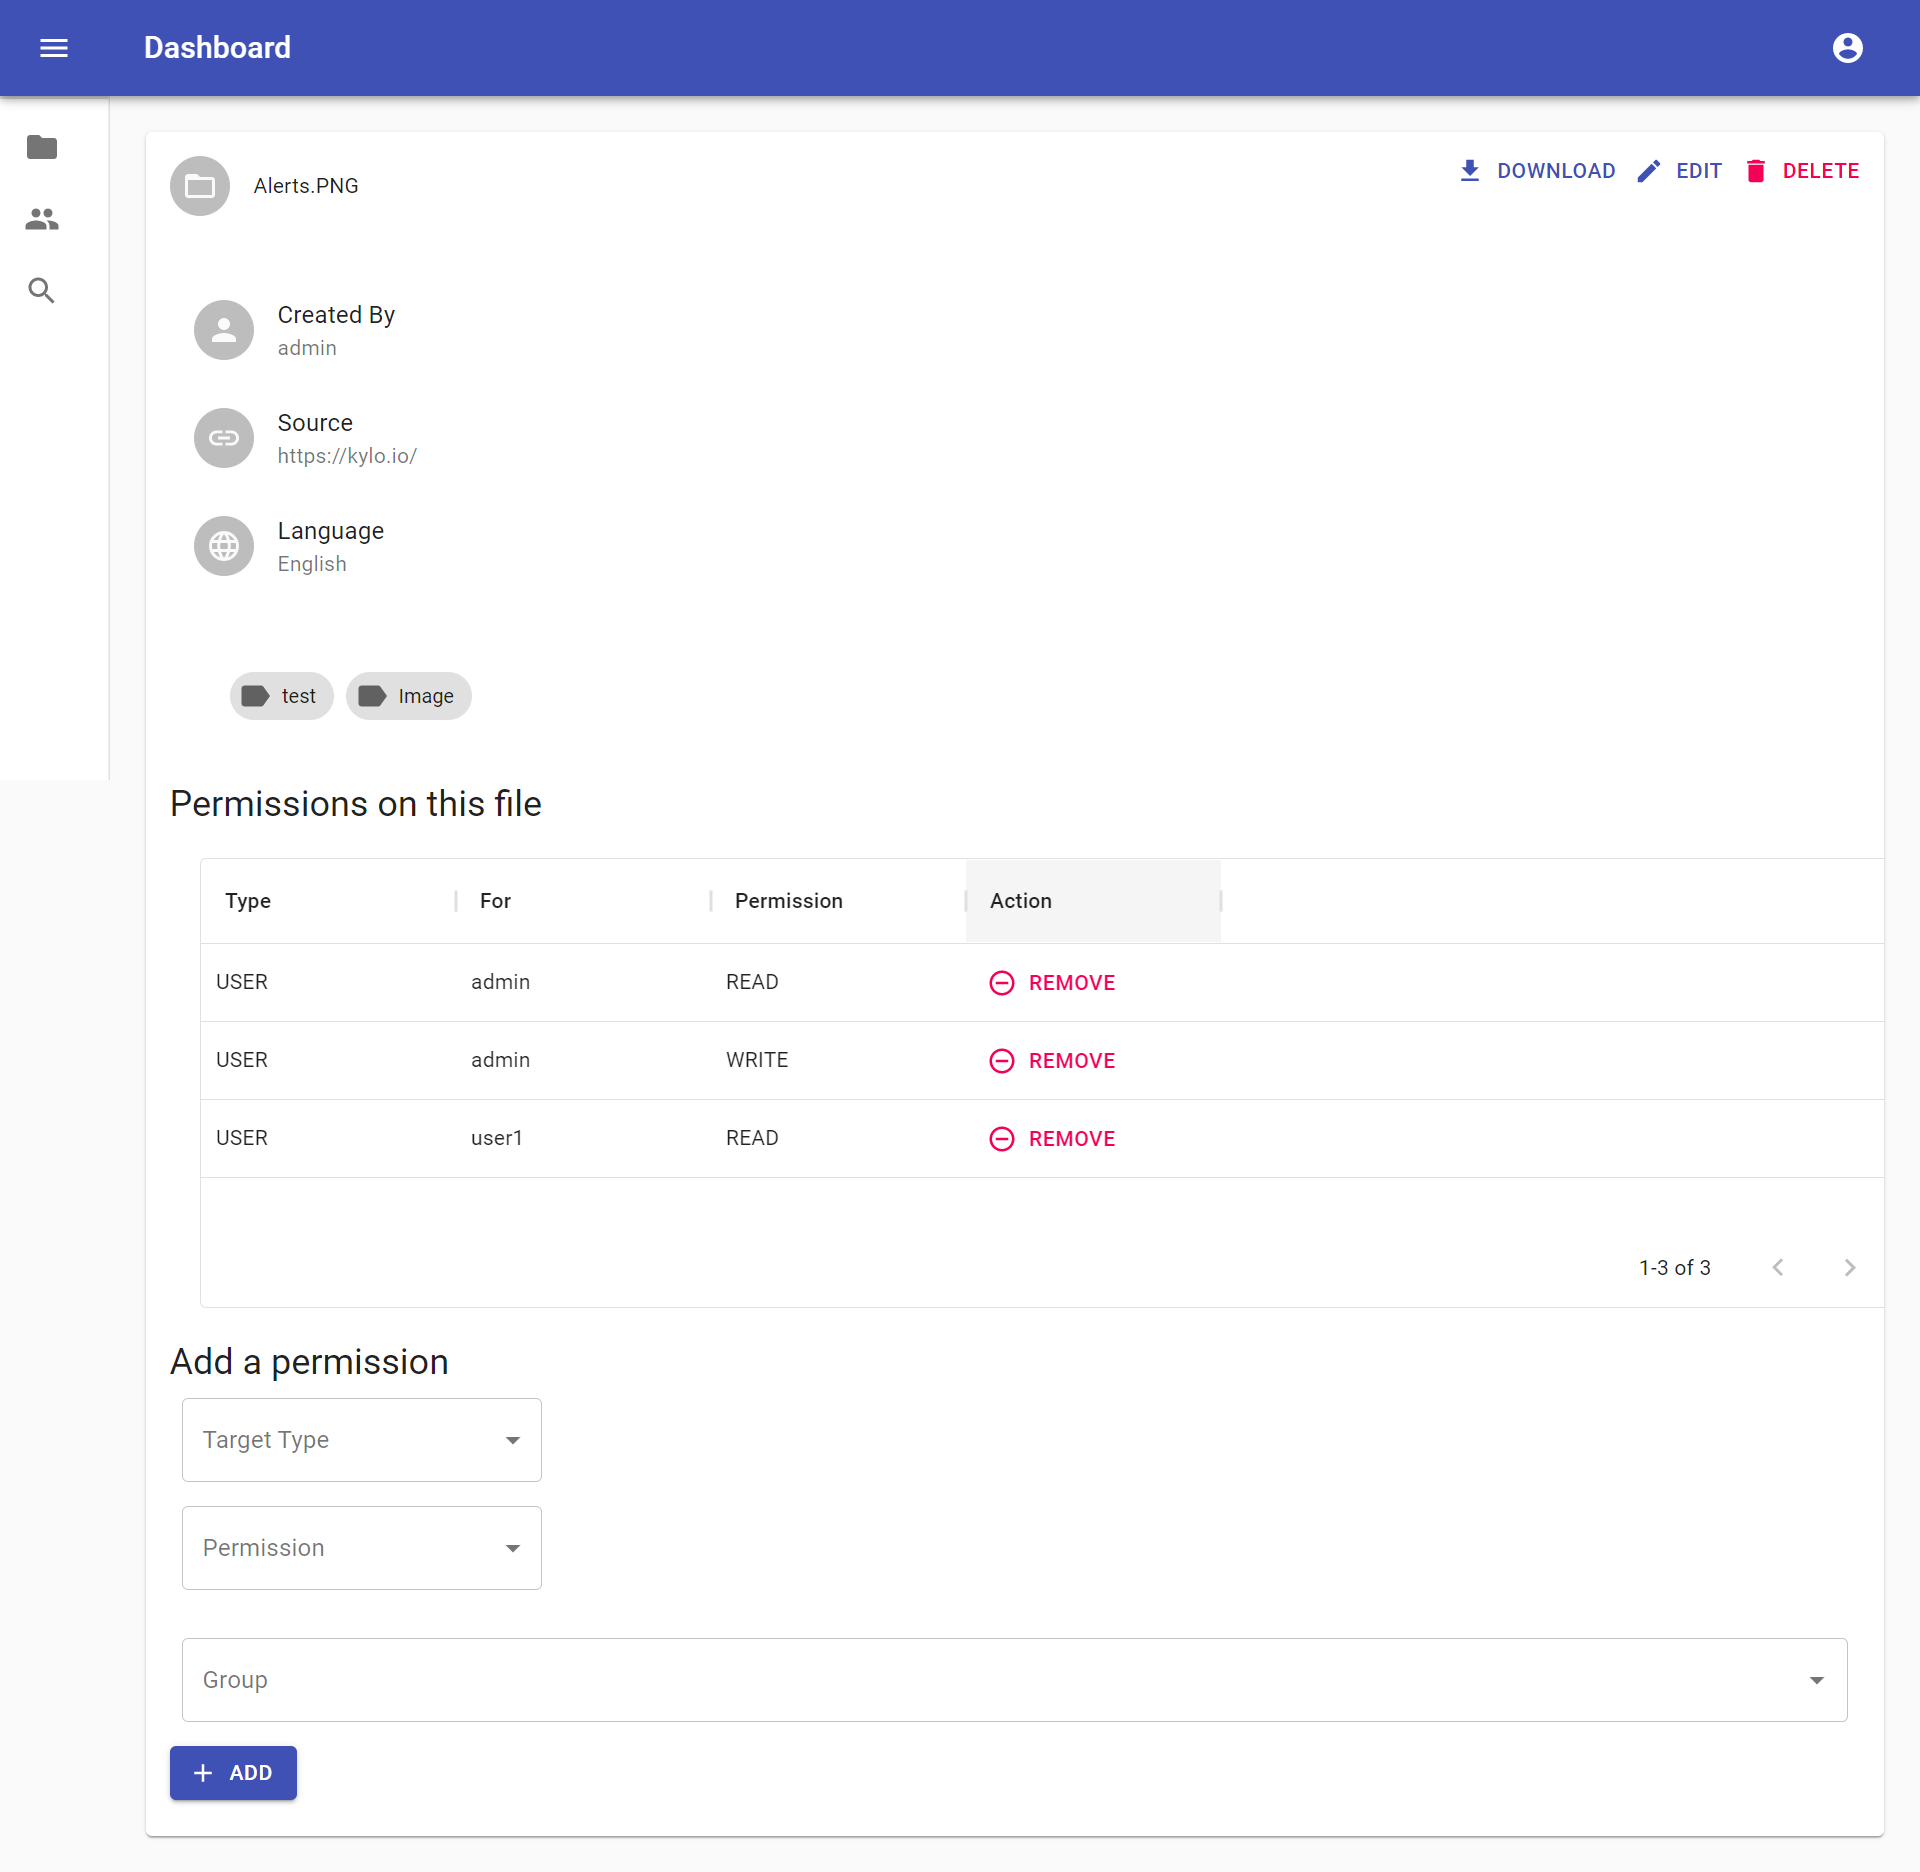
\includegraphics[width=1.0\textwidth]{images/File-ViewDetails.png}
    \caption{View File Details user interface}
    \label{fig:viewFile}
\end{figure}
\begin{figure}[H]
    \centering
    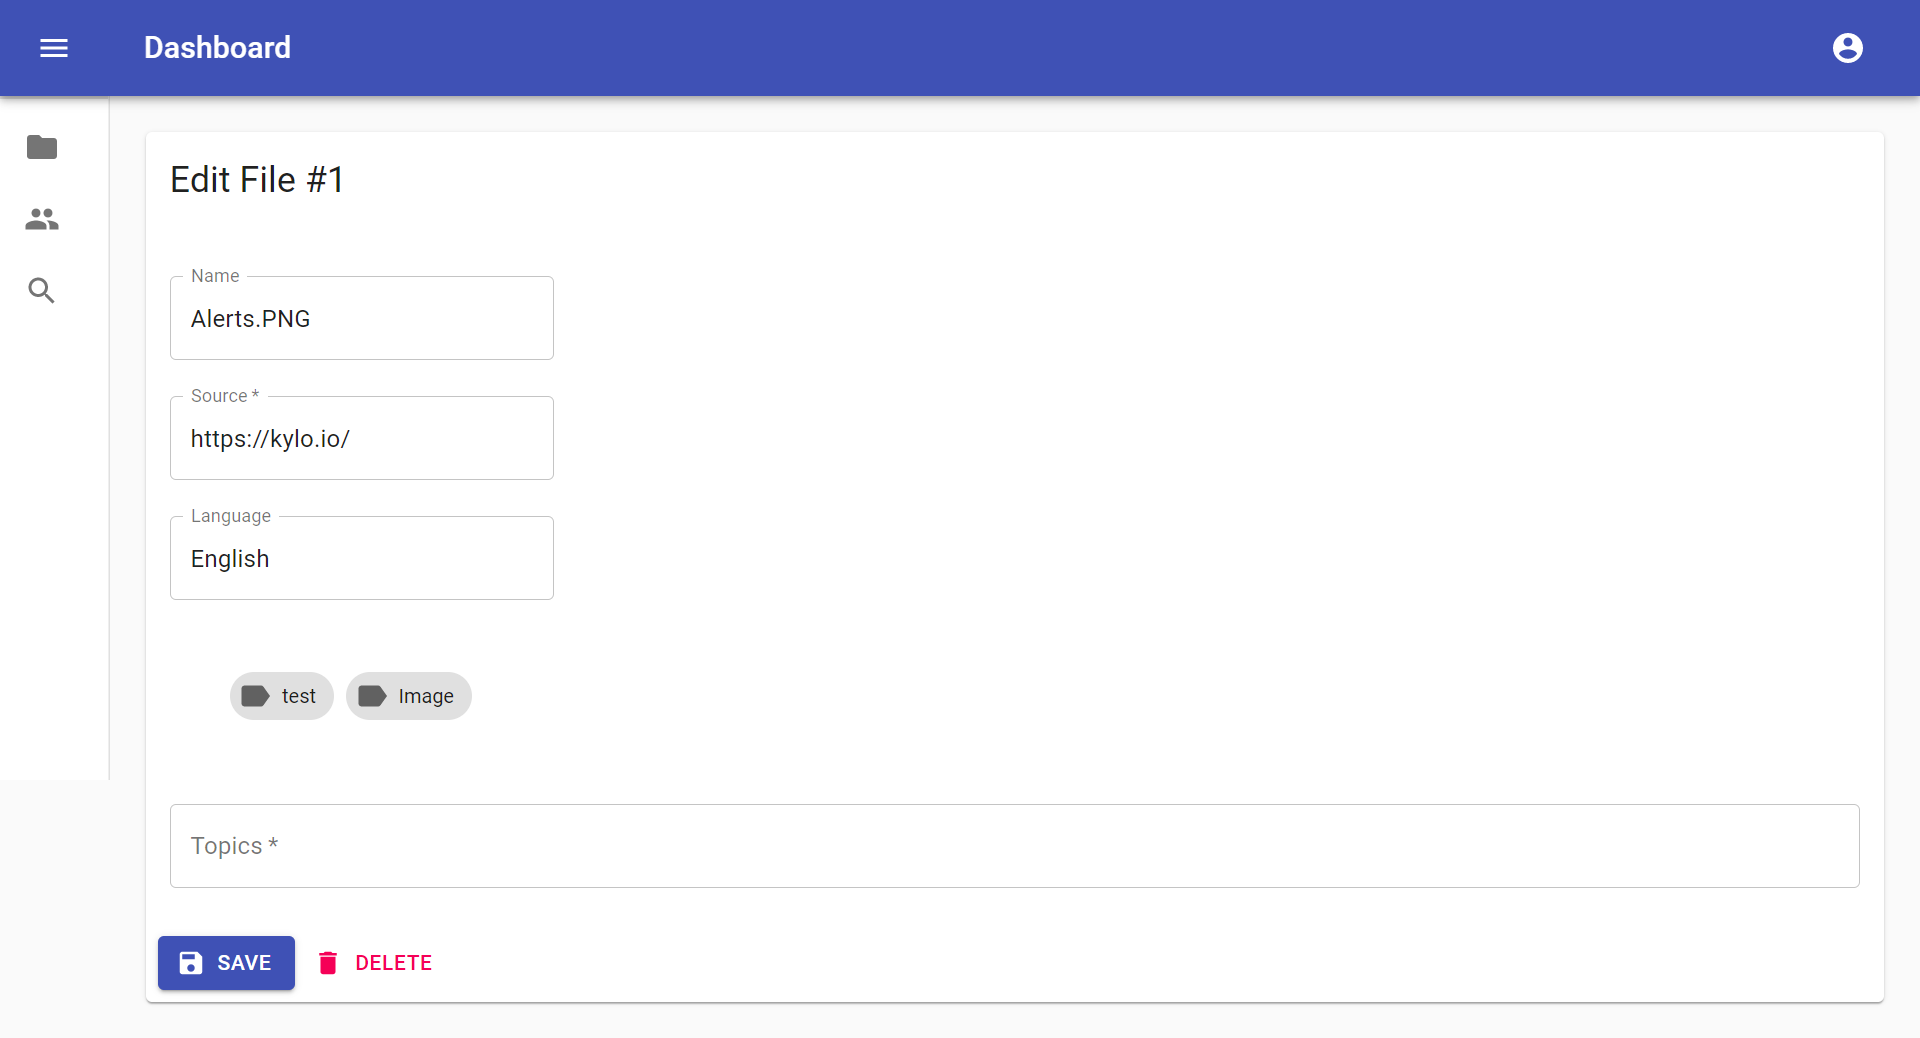
\includegraphics[width=1.0\textwidth]{images/File-Edit.png}
    \caption{Edit File user interface}
    \label{fig:editFile}
\end{figure}
\section{Discussion}
Despite being implemented completely, the main functions in this project have some existing
problems. 

The concept of Data Lake is new to us. And it takes a long time to get a sense of what it is and how to do.

Furthermore, because this website was not created by a team of experienced creators but by a novice individual, it contains numerous flaws in terms of design and features.

Finally, time constraints prevent the testing process from being completed completely and methodically, potentially resulting in a large number of minor problems. On the other hand, this website has accomplished all of the initial objectives listed in the Objectives chapter.